\providecommand{\main}{../../..}
\documentclass[\main/main.tex]{subfiles}
\begin{document}

\subsection{Exercise 3}
The following table holds values of 5 solutions with 2 cost criteria:
\begin{table}
  \begin{tabular}{L|LLLLL}
        & a_1 & a_2 & a_3 & a_4 & a_5 \\
    \hline
    f_1 & 20  & 60  & 30  & 50  & 100 \\
    f_2 & 70  & 20  & 30  & 40  & 0
  \end{tabular}
\end{table}

\begin{enumerate}[a)]
  \item Determine if there are dominated alternatives.
  \item Determine the paretian frontier with the constraints method.
  \item Determine the supported solutions and the support for each one.
\end{enumerate}

\subsection{Exercise 3 resolution}
\subsubsection*{a) Dominated alternatives}
The solution $a_3$ dominates $a_4$.

\subsubsection*{Constraints method}
First of all we plot the points on the $f_1-f_2$ plane:

\begin{figure}
  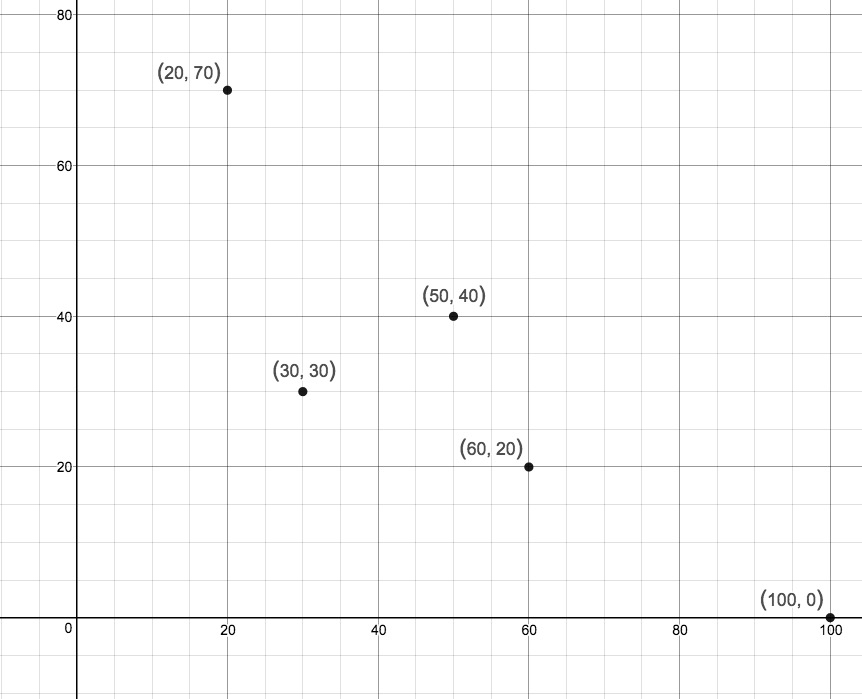
\includegraphics[width=0.4\textwidth]{20180124_03_1}
\end{figure}

Since it's a minimization problem (the indicator values are costs), the standard function will be of the kind: $f_1 \leq \epsilon$.

There are no solution for the standard $\epsilon < 20$, so it holds no interest.

\begin{figure}
  \begin{subfigure}{0.32\textwidth}
    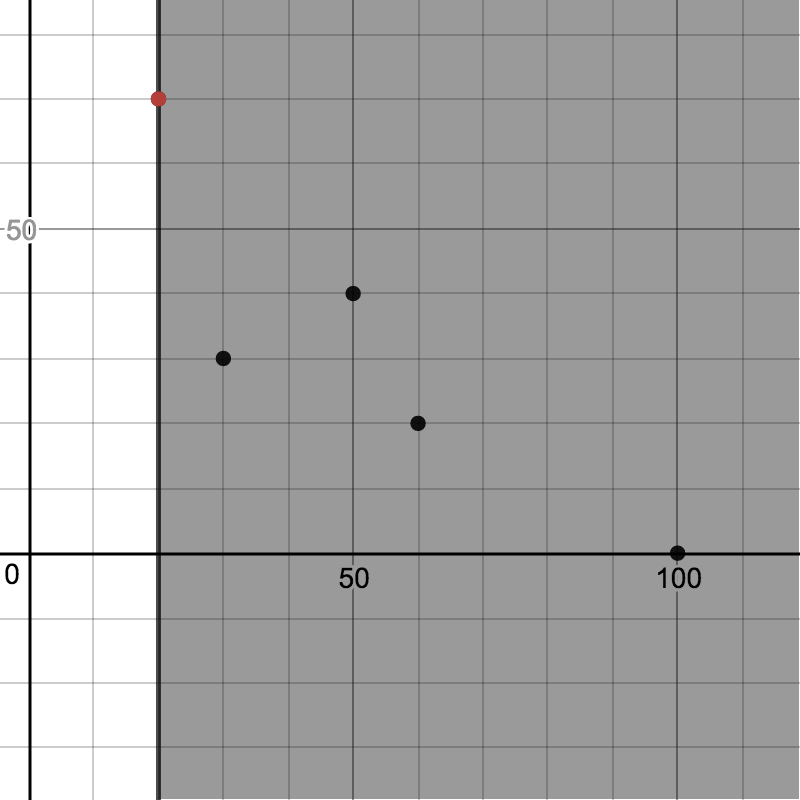
\includegraphics[width=\textwidth]{20180124_03_2}
    \caption{$\epsilon=20$, $f_1 \leq 20$, optimal solution $a_1$}
  \end{subfigure}
  \begin{subfigure}{0.32\textwidth}
    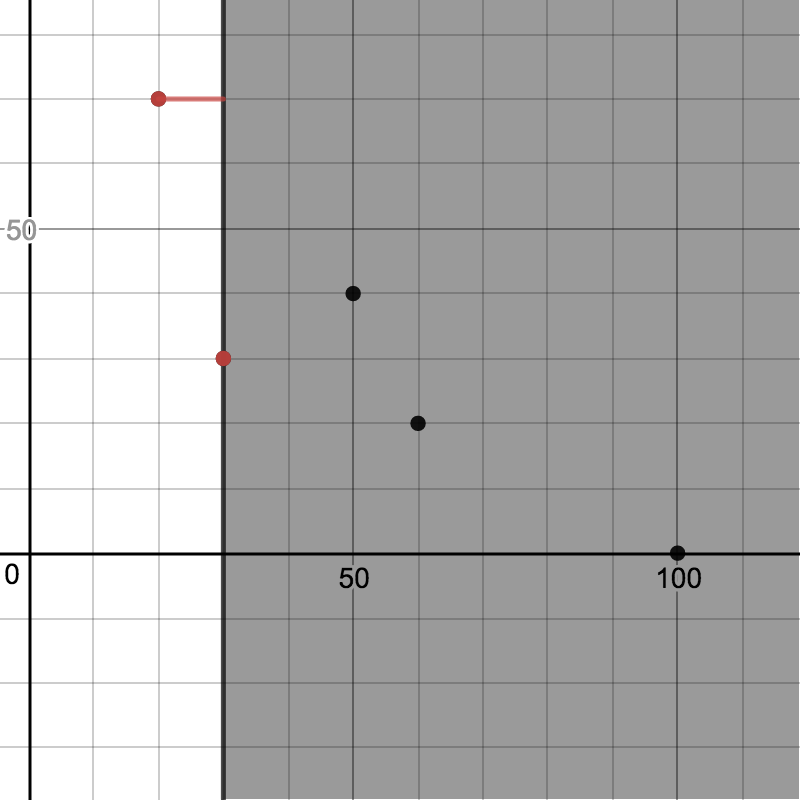
\includegraphics[width=\textwidth]{20180124_03_3}
    \caption{$\epsilon=30$, $f_1 \leq 30$, optimal solution $a_3$}
  \end{subfigure}
  \begin{subfigure}{0.32\textwidth}
    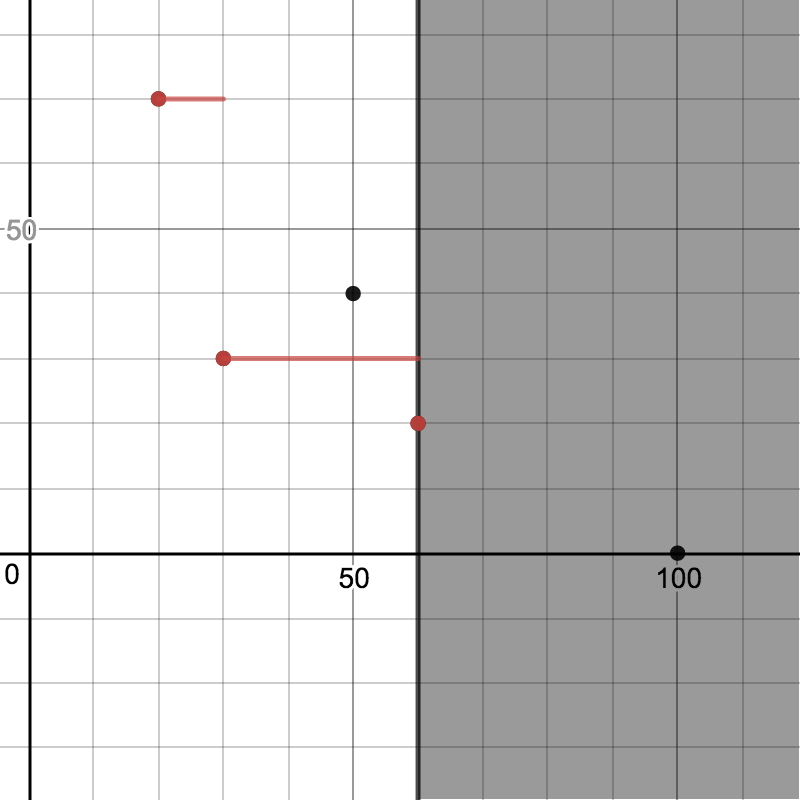
\includegraphics[width=\textwidth]{20180124_03_4}
    \caption{$\epsilon=60$, $f_1 \leq 60$, optimal solution $a_2$}
  \end{subfigure}
  \begin{subfigure}{0.32\textwidth}
    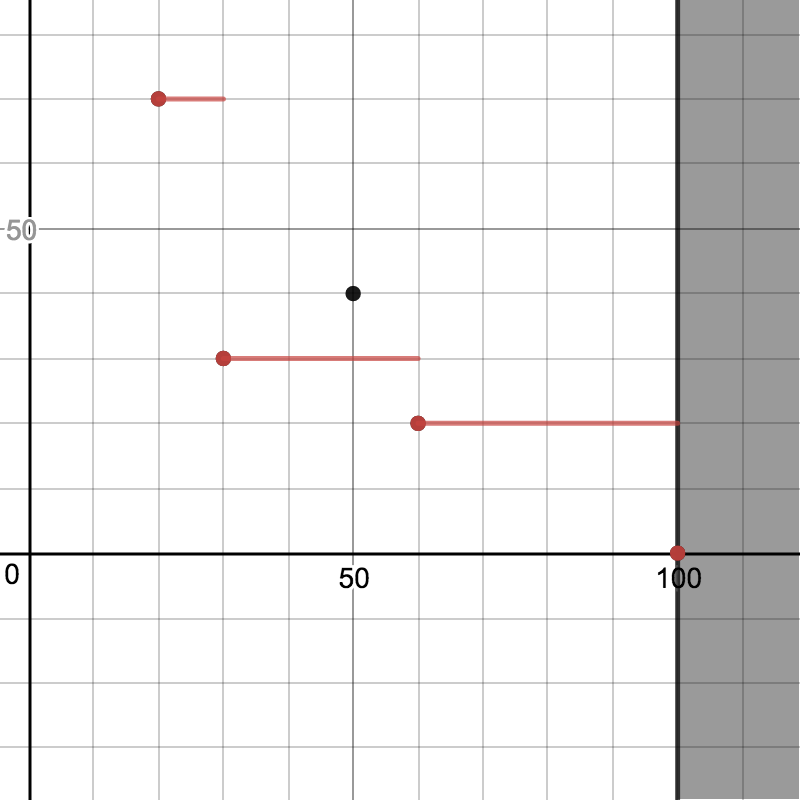
\includegraphics[width=\textwidth]{20180124_03_5}
    \caption{$\epsilon=100$, $f_1 \leq 100$, optimal solution $a_5$}
  \end{subfigure}
  \begin{subfigure}{0.32\textwidth}
    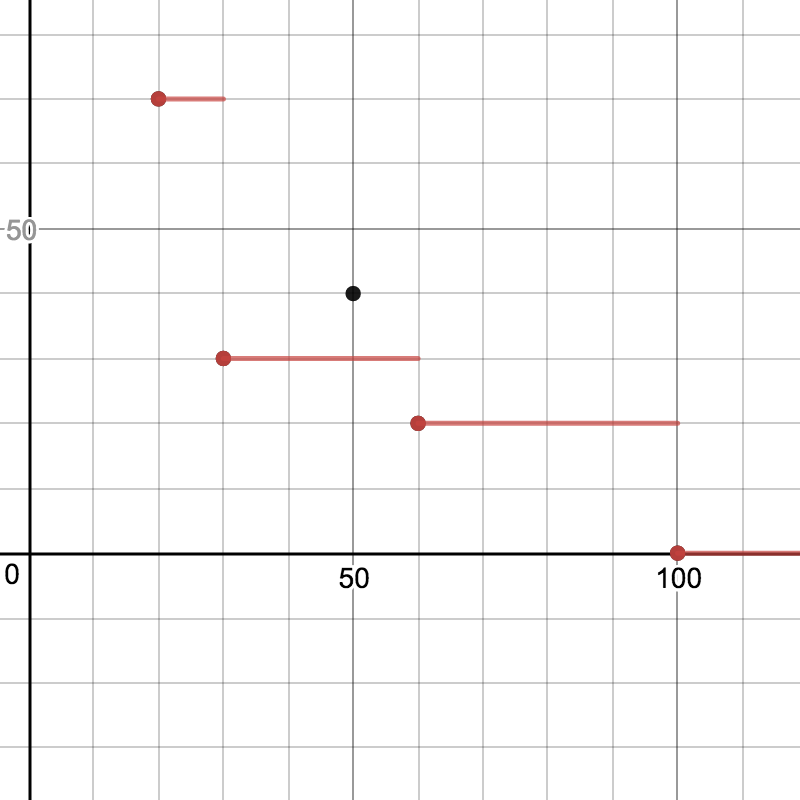
\includegraphics[width=\textwidth]{20180124_03_6}
    \caption{$\epsilon=\infty$, $f_1 \leq \infty$, optimal solution $a_5$}
  \end{subfigure}
  \caption{Paretian frontier}
\end{figure}

\subsubsection*{Solutions support}
Let's define $\w_1$ as the weight for the indicator $f_1$ and $\w_2 = 1-\w_1$ for the indicator $\w_2$.

\begin{figure}
  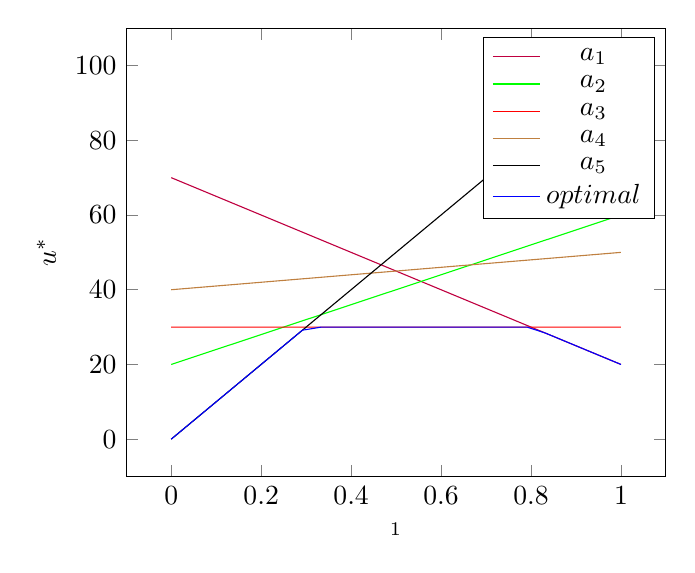
\begin{tikzpicture}
    \begin{axis}[
        xlabel=$\w_1$,
        ylabel=$u^*$,
        domain=0:1
      ]
      \addplot[mark=none,color=purple]{
        20*x+70*(1-x)
      };
      \addplot[mark=none,color=green]{
        60*x+20*(1-x)
      };
      \addplot[mark=none,color=red]{
        30*x+30*(1-x)
      };
      \addplot[mark=none,color=brown]{
        50*x+40*(1-x)
      };
      \addplot[mark=none,color=black]{
        100*x+0*(1-x)
      };
      \addplot[mark=none,color=blue]{
        min(min(min(min(
        20*x+70*(1-x),
        60*x+20*(1-x)
        ),
        30*x+30*(1-x)
        ),
        50*x+40*(1-x)
        ),
        100*x+0*(1-x)
        )
      };
      \legend{$a_1$, $a_2$, $a_3$, $a_4$, $a_5$, $optimal$}
    \end{axis}
  \end{tikzpicture}
  \caption{Supports}
\end{figure}

For $\w_1 \leq \frac{3}{10}$ the optimal solution is $a_5$.

For $\frac{3}{10} \leq \w_1 \leq \frac{4}{5}$ the optimal solution is $a_3$.

For $\w_1 \geq \frac{4}{5}$ the optimal solution is $a_1$.

\end{document}